\chapter{Traduction, Compilation, interprétation}

\section{Langage bas niveau : Assembleur}

Je pense que vous serez d'accord sur le fait que programmer une machine en langage machine (1000 1C00 ) n'est pas très confortable. Au delà du fait que ce ne soit pas très confortable, cette forme de programmation est tellement proche de l'architecture matérielle qu'elle n'autorise pas des évolutions du matériel sans modification du programme. Le langage d'assemblage permet de se détacher du langage machine et donc de l'implémentation matérielle tout en offrant une plus grande simplicité de programmation. Le langage d'assemblage est constitué de mnémoniques pour les instructions. Par exemple, avec l'architecture que nous utilisons en TP, vous trouverez sur la figure\ref{fig:codemachine_asm} un programme écrit en langage machine et son équivalent en langage d'assemblage\footnote{par abus de langage, plutôt que de parler de langage d'assemblage, on parle d'assembleur. En toute rigueur, l'assembleur est le programme qui traduit le language d'assemblage en language machine.}. Le programme en langage d'assemblage est plus facile à lire et à écrire et on voit sur cet exemple l'utilisation d'une étiquette (sum) pour désigner l'adresse de la routine dont la valeur est calculée par le programme traduisant le programme en code machine.

\begin{figure}[htbp]
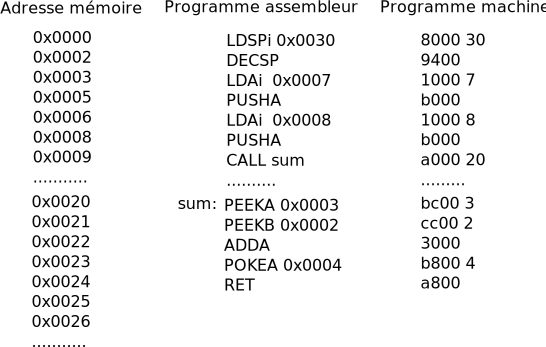
\includegraphics[width=0.7\linewidth]{Figs/traduction_asm_machine_call.pdf}
\caption{\label{fig:codemachine_asm} Code machine et code assembleur d'un programme. Il est plus facile d'écrire et de comprendre un programme en langage d'assemblage qu'en code machine. Le langage d'assemblage ajoute également quelques fonctionnalités comme par exemple l'utilisation d'étiquette (sum) dont la valeur est calculée par l'assembleur.}
\end{figure}

La programmation en langage machine est assez fastidieuse pour plusieurs raisons 
\begin{itemize}
\item il faut se souvenir des codes machines (0x10, 0x14, ..) des instructions qu'il est plus difficile de retenir que les "mnémoniques" (LDAi, LDAd, ...)
\item il faut calculer à la main les adresses lors des branchements alors qu'on pourrait baliser un programme d'étiquettes qu'un assembleur réécrirait
\item il faut déterminer à la main les adresses ou stocker la pile, les variables globales, .... alors qu'un programme pourrait déterminer l'agencement de la mémoire automatiquement au regard de la taille du programme.
\end{itemize}

\subsection{Quelques éléments de syntaxe de notre langage d'assemblage}

Je vous propose dans cette partie d'introduire un langage d'assemblage pour la machine que nous utilisons en TP. Le programme en langage d'assemblage est écrit avec les mnémoniques de la façon suivante :

\begin{verbatim}
LDAi 3
STA  1001
...
\end{verbatim}

Chaque ligne contient au plus une instruction. Les valeurs qui suivent les instructions doivent être hexadécimales (on ne les préfixe pas par 0x). Le langage d'assemblage accepte les commentaires, préfixés de ";" :

\begin{verbatim}
LDAi 3  ; ceci est un commentaire : on charge 3 dans le registre A
\end{verbatim}

On peut utiliser des étiquettes pour référencer des lignes du programme :

\begin{verbatim}
init: LDSPi @stack@
      LDAi 1
      LDBi 1
loop: ADDA
      STA  1001
      JMP loop
\end{verbatim}

Le mot clef "@stack@" est réservé par le langage : c'est le programme traduisant le programme qui calculera automatiquement l'adresse mémoire ou débute la pile. Si vous avez besoin de stocker des variables globales en mémoire, vous utiliserez l'instruction DSW qui réserve un mot mémoire et lui associe une étiquette :

 \begin{verbatim}
  DSW compteur
  LDAi 0
  STA  compteur
\end{verbatim}

Par convention, on allouera les variables globales au début du programme. Il est interdit d'utiliser des noms de variable ou des étiquettes qui peuvent s'interpréter comme une valeur hexadécimale. Par exemple, vous ne pouvez pas écrire

\begin{verbatim}
DSW ff ; interdit
\end{verbatim}

%\subsection{D'autres éléments de langage d'assemblage}
%
%\begin{itemize}
%\item les macros
%\end{itemize}




\subsection{L'assembleur}

\subsubsection{Compteur d'emplacement et table des symboles}

Le programme écrit en langage d'assemblage n'est évidemment pas compréhensible par la machine qui ne comprends que des séquences binaires ! Il faut donc traduire le programme écrit en langage d'assemblage en code machine; c'est le rôle d'un programme qu'on appelle l'assembleur. L'assembleur est en général l'un des premiers programmes écrit pour une architecture étant donnée la souplesse qu'il offre pour l'écriture de programmes. Un programme source en assembleur peut presque se traduire ligne par ligne en code machine. Pourquoi presque ? Considérons le programme de la figure \ref{fig:codemachine_asm}. Lorsqu'on souhaite traduire la ligne invoquant la routine ``CALL sum'', il faut savoir par quelle valeur remplacer l'étiquette sum. Mais comme la routine est définie plus tard dans le programme, on ne sait pas encore quelle sera cette valeur : c'est ce qu'on appelle une référence en avant. Pour résoudre les références, on introduit la \textbf{table des symboles} qui fait correspondre à chaque étiquette sa valeur. Pour savoir quelle valeur attribuer à l'étiquette sum lorsqu'on la rencontre, on introduit un compteur, le compteur d'emplacement, qui sera incrémenté chaque fois qu'une instruction ou une opérande est rencontrée et, lorsqu'on rencontre une étiquette, on sauvegarde dans la table des symboles la valeur de ce compteur. Notre assembleur fonctionne donc en deux passes : dans une première passe, l'assembleur collecte les symboles et leur valeur et dans une deuxième passe utilise le programme source en assembleur, le code des instructions et la table des symboles pour produire le code machine. Par exemple, supposons que nous souhaitions traduire le programme ci-dessous :

\begin{verbatim}
      LDAi 1
      LDBi 1
loop: ADDA
      STA 1001
      JMP loop
\end{verbatim}

Le tableau ci-dessous donne l'évolution du compteur d'emplacement et de la table des symboles lors de la première passe de l'assembleur. Toutes les valeurs sont à considérer en hexadécimal. La table des symboles indique donc que l'étiquette loop corresponds à l'adresse en mémoire $0\times0004$.

\begin{tabular}{cc}
\begin{tabular}{c|c|c|c}
Etiquette & Instruction& Opérande & Compteur d'emplacement\\
\hline
& LDAi & 1 & 0 $\rightarrow$ 2\\
& LDBi & 1 & 2 $\rightarrow$ 4\\
loop & ADDA & & 4 $\rightarrow$ 5\\
& STA & 1001 & 5 $\rightarrow$ 7\\
& JMP & loop & 7 $\rightarrow$ 9
\end{tabular}&
\begin{tabular}{c|c}
Symbole & Valeur\\
\hline
loop & 4
\end{tabular}
\end{tabular}

Une fois la table des symboles remplie, la deuxième passe de l'assemblage peut remplacer chaque ligne par son code binaire en utilisant le code des instructions.

\begin{minipage}{0.4\linewidth}
\begin{verbatim}
      LDAi 1
      LDBi 1
loop: ADDA
      STA 1001
      JMP loop
\end{verbatim}
\end{minipage}
$\Rightarrow$
\hfill
\begin{minipage}{0.4\linewidth}
\begin{verbatim}
1000 0001
2000 0001
3000
1C00 1001
7000 0004
\end{verbatim}
\end{minipage}

\subsubsection{Organisation de la mémoire}

Pour notre architecture, on ne s'autorise à utiliser que la plage d'adresse [0x0000, 0x0FFF] pour stocker le programme et les données (la pile par exemple). Les adresses supérieures à 0x1000 sont réservées pour les entrées/sorties dont on reparlera dans le prochain chapitre. Si des variables globales sont déclarées dans le programme \texttt{DSW}, elles se voient affectée des emplacements em mémoire à partir de l'adresse 0x0FFF, vers les adresses décroissantes. Une fois toutes les variables globales stockées en mémoire, l'assembleur place la pile. Le pointeur de pile est donc calculé automatiquement par l'assembleur en décrémentant l'adresse 0x0FFF du nombre de variables globales. Schématiquement, cela donne une organisation mémoire représentée sur la figure \ref{fig:mem_layout}.

\begin{figure}[htbp]
\centering\includegraphics[width=0.25\linewidth]{Figs/mem_layout.pdf}
\caption{\label{fig:mem_layout} Organisation mémoire pour notre architecture. Seules les adresses [0,0000, 0x0FFF] sont utilisables pour le programme et les données. Les variables globales déclarées par la pseudo instruction DSW sont placées à la fin de ce ségment et la pile juste avant. L'assembleur affecte automatiquement le placement de la pile @stack@ en tenant compte du nombre de variables globales déclarées. }
\end{figure}

\subsubsection{Pourquoi aller plus loin ?}

Malgré le coup de pouce qu'apporte un langage d'assemblage, il reste encore quelques inconvénients :
\begin{itemize}
\item on reste dépendant du jeu d'instruction d'une architecture,
\item la programmation en assembleur reste encore difficile et n'est pas suffisamment intelligible
\item on doit allouer soit même les registres
\end{itemize}

Pour illustrer le deuxième point, je vous propose ci-dessous un programme écrit en Python et sa possible écriture avec notre langage d'assemblage :

\begin{minipage}{0.4\linewidth}
\begin{verbatim}
n = 0
i = 0
while(i != 5):
    n = n + i
    i = i + 1
\end{verbatim}
\end{minipage}
\hfill
\begin{minipage}{0.4\linewidth}
\begin{verbatim}
      DSW n
      DSW i
      LDAi 0
      STA n      ; n = 0
      LDAi 0 
      STA i      ; i = 0
loop: LDAd i
      LDBi 5
      SUBA
      JZA endl   ; i !=  5 ?
      LDAd n
      LDBd i
      ADDA
      STA n      ; n = n + i
      LDAd i
      LDBi 1
      ADDA   
      STA i      ; i = i + 1
      JMP loop
endl: END
\end{verbatim}
\end{minipage}



\section{Langage de haut niveau}


\subsection{Quelques éléments de langages de haut niveau}

Les langages de haut niveau tels que C, C++, Java, Python, ... apporte une plus grande facilité de programmation des machines en fournissant par exemple :
\begin{itemize}
\item des éléments de syntaxe : tests conditionnels ``if() else if ..'', boucles ``for i in ..'', ``x = 1 + 2'', ..
\item une allocation automatique des registres, et des emplacements mémoires ``x = 3'', ``x + y''
\item une optimisation du code par exemple en disposant de manière optimiale des portions du programme pour minimiser le nombre de branchement
\item des contraintes sur les opératons applicables sur les variables en les typant
\end{itemize}


\subsection{Interprété ou compilé}

Le langage d'assemblage offre une certaine facilité pour écrire des programmes mais ce n'est pas encore l'idéal. Etant donné l'exemple donné précédemment, vous serez d'accord, je pense, que le programme écrit en python est beaucoup plus facilement compréhensible (en plus d'être nettement plus court) que le programme écrit en langage d'assemblage. Les langages comme python, C, C++, java, etc.. sont ce qu'on appelle des langages de haut niveau. Ces langages \textbf{ne font plus appel au jeu d'instruction d'une architecture} et c'est en ce sens qu'ils sont de haut niveau, ils offrent une couche d'abstraction supplémentaire qui permet de se détacher de la réalisation matérielle de la machine. Pour le coup, ce sera exactement le même programme C/C++ qui sera utilisé sur une machine Intel x86 ou ARM, pourvu que vous disposiez d'un programme qui puisse d'une manière ou d'une autre exécuter le programme écrit dans ce langage de haut niveau. On distingue deux principales approches : les langages interprétés et les langages compilés. Les langages interprétés, comme Python, sont évalués par un programme qu'on appelle interpréteur. L'interpréteur est écrit en code machine et exécute le programme que vous avez écrit. Contrairement aux langages interprétés qui sont ``directement'' exécuté sur une machine en étant interprété par un programme (l'interpréteur), un langage compilé nécessite une première étape, dite de compilation, qui transforme le code en code machine puis une deuxième étape, dite d'exécution.


%\url{http://akaptur.com/blog/2013/11/15/introduction-to-the-python-interpreter/}, \url{http://tomlee.co/wp-content/uploads/2012/11/108_python-language-internals.pdf}
%\todo{Lexing, parsing, compiling, interpreting}


\section{Compilateur}

\subsection{Anatomie d'un compilateur}

Un compilateur est un programme exécutable sur une architecture qui prends en argument un programme source (texte) et produit comme résultat un code binaire pour une architecture spécifique (utilisant les instructions et leur code d'une machine donnée) : ce sont les compilateurs qui, partant d'un programme source identique produisent des programmes différents en code machine pour chaque architecture. D'un point de vue général, le processus de compilation se déroule en deux étapes : l'analyse et la synthèse (fig.\ref{fig:compilation_frontend_backend}). La phase d'analyse est réalisée par ce qu'on appelle un \emph{frontend} et la phase de synthèse par ce qu'on appelle un \emph{backend}.

\begin{figure}[htbp]
\includegraphics[width=\linewidth]{Figs/compilation_frontend_backend.pdf}
\caption{\label{fig:compilation_frontend_backend} Le compilateur est un programme transformant un programme source en un programme en code machine pour une architecture ciblée. Il est construit en deux phases : le frontend très spécifique à un langage donné qui produit un programme en un certain langage intermédiaire (e.g. un graphe de flot de contrôle) et le backend relativement générique qui produit le code machine à partir de la représentation intermédiaire.}
\end{figure}

La phase d'analyse est réalisée par un frontend très dépendant du langage source (C, C++, Scala, ..) qui transforme le programme source en un langage intermédiaire. La phase de synthèse transforme le programme en langage intermédiaire en un code machine et cette phase est réalisée par un \emph{backend} très dépendant de l'architecture cible mais relativement indépendant du langage source. L'avantage de cette construction est qu'une partie du travail (frontend) est langage source dépendant, tandis qu'une autre est machine cible dépendant. Si on souhaite définir un nouveau langage, il suffit d'écrire un frontend, et les backends existants pourront être utilisés pour produire du code machine pour plusieurs architectures. Si on se définit une nouvelle architecture, il suffit d'écrire la partie backend pour notre architecture et utiliser les frontend des langages de haut niveau déjà développés. Je vous propose dans les parties qui suivent un bref aperçu des différentes étapes de compilation et vous propose de vous référer à \cite{DragonBook} pour plus de détails.

\subsection{La phase d'analyse (frontend)}

Le programme source étant du texte en mémoire, la première étape de la phase d'analyse consiste à ségmenter ce texte en éléments constitutifs identifiés (on parle aussi d'analyse lexicale). Pour réaliser cette analyse lexicale, on utilise un lexique, qui permet par exemple de reconnaître des mots du langage ``for'', ``if'', ``while'' ou bien que ``1234'' est une constante entière etc.. Par exemple, sur la figure \ref{fig:lexing}, le programme écrit en C est ségmenté et chacune des pièces du puzzle est identifiée. On obtient à l'issu de la phase d'analyse lexicale une liste de lexèmes.

\begin{figure}[htbp]
\includegraphics[width=0.5\linewidth]{Figs/lexing.pdf}
\caption{\label{fig:lexing}L'analyse lexicale transforme le texte du programme en une séquence d'éléments identifiés (lexéme ou \emph{tokens}).}
\end{figure}

La deuxième étape de la phase d'analyse consiste à s'assurer que le programme est syntaxiquement correct en travaillant à partir de la liste des lexèmes. Connaissant le type de chacun des éléments ségmentés, on peut par exemple s'assurer qu'un opérateur binaire met bien en relation deux opérandes; par exemple, le programme ``int x = y +;'' est syntaxiquement incorrect puisqu'il manque une opérande à l'opérateur binaire ``+''. Les compilateurs modernes fournissent des retours à l'utilisateur, notamment lors d'une erreur de syntaxe. Par exemple, si je tente de compiler le programme C++ de la figure \ref{fig:erreur_syntaxe} avec le compilateur GNU GCC, celui ci m'affiche non seulement qu'il y a une erreur de syntaxe mais également la ligne à laquelle cette erreur se présente.

\begin{figure}[htbp]
\centering\includegraphics[width=0.6\linewidth]{Figs/erreur_syntaxe.pdf}
\caption{\label{fig:erreur_syntaxe} Lors de la phase d'analyse syntaxique, le compilateur peut détecter des erreurs de syntaxe et les indiquer à l'utilisateur le cas échéant. Ici, nous avons un exemple d'un programme C contenant une erreur de syntaxe que le compilateur GNU gcc a détecté.}
\end{figure}


L'analyse syntaxique se déroule en construisant, à partir des lexèmes, un arbre syntaxique comme illustré sur l'exemple de la figure \ref{fig:syntactic_tree} qu'on appelle un arbre syntaxique abstrait. La construction de cet arbre syntaxique est réalisée grâce à une grammaire d'un langage donné qui spécifie la manière dont les lexèmes peuvent être combinés pour donner des phrases ou des expressions valides.

\begin{figure}[htbp]
\includegraphics[width=\linewidth]{Figs/syntactic_tree.pdf}
\caption{\label{fig:syntactic_tree} A partir du résultat de l'analyse lexicale, l'analyse syntaxique construit un arbre syntaxique et s'assure au passage que la syntaxe du langage est respectée. Par exemple, la construction ``int x = y + ;'' est syntaxiquement incorrecte en C.}
\end{figure}

La phase d'analyse se termine par l'analyse sémantique. Cette dernière étape vérifie essentiellement que les opérations mettent en relation les bons types; par exemple, en C++, il est interdit d'écrire ``int x = 1+"toto";'';



Pour résumer, la phase d'analyse se déroule en plusieurs étapes :
\begin{itemize}
\item une analyse lexicale qui ségmente le texte du programme en éléments identifiés
\item une analyse syntaxique qui vérifie si la construction du programme est syntaxiquement correcte
\item une analyse sémantique qui garantie par exemple que les variables utilisées dans des expressions ont le bon type
\end{itemize}
A l'issue de cette phase d'analyse, on obtient une représentation intermédiaire du programme dans un certain formalisme comme un graphe de flot de contrôle.

\subsection{Génération et optimisation d'une représentation intermédiaire}

% Examples de TAC : http://dound.com/courses/cs143/handouts/17-TAC-Examples.pdf
% Optimisation d'un CFG en TAC : http://www.csd.uwo.ca/~moreno//CS447/Lectures/CodeOptimization.html/node2.html

Après la phase d'analyse, le programme est traduit dans ce qu'on appelle un langage intermédiaire. Le but de ce langage intermédiaire est :
\begin{enumerate}
\item d'offrir une représentation qui soit indépendante du langage source (e.g. C, C++) et l'architecture cible (x86, ARM) servant ainsi de médiateur entre ces deux mondes et facilitant le développement de compilateurs pour de nouveaux langages ou de nouvelles architectures
\item d'offrir une représentation qui permette d'effectuer un certain nombre d'optimisation
\end{enumerate}
Il existe plusieurs représentations internes (\emph{Register transfer language}, \emph{gimple}, \emph{generic}, \emph{three adress code}, \emph{single static assignment}, \emph{control flow graph}). Considérons par exemple le code à trois adresse. Ce langage contient des constructions comme :
\begin{itemize}
\item des affectations de résultat d'opérateurs binaires : [x := y op z]
\item des affectations de résultat d'opérateur unaire : [x := op y]
\item des copies : [x := y]
\item des branchements inconditionnels [goto L]
\item des tests conditionnels [IfZ x Goto L]
\item ...
\end{itemize}

La figure ci-dessous illustre la construction intermédiaire d'un programme écrit en C, en son équivalent en code à trois adresses:
\lstset { %
    language=C++,
    backgroundcolor=\color{black!5}, % set backgroundcolor
    basicstyle=\footnotesize,% basic font setting
}

\begin{minipage}[c]{0.4\linewidth}
\begin{lstlisting}
int x = 3;
int y = 2 + 7 + x;
int z = 2*y;
if(x < y) {
  z = x/2 + y/3;
}
else {
  z = x * y + y;
}
\end{lstlisting}
\end{minipage}
\begin{minipage}[c]{0.5\linewidth}
\begin{verbatim}
     x = 3;
     _t1 = 2 + 7;
     y = _t1 + x;
     z = 2 * y;
     _t2 = x < y;
     IfZ _t2 Goto _L0;
     _t3 = x / 2;
     _t4 = y / 3;
     z = _t3 + _t4
     Goto _L1
_L0: _t5 = x * y;
     z = _t5 + z;
_L1:
\end{verbatim}
\end{minipage}

L'avantage du code à trois adresses est qu'il facilite l'optimisation du code comme la détection de variables non utilisées\footnote{qu'on apprécierait en fait mieux si on utilisait la représentation de \emph{single static assignement}}. Ce code à trois adresse est structuré sous la forme d'un graphe de flot de contrôle. Un graphe de flot de contrôle représente un programme sous la forme de blocs qui contiennent des affectations et se terminent éventuellement par un saut. La figure \ref{fig:control_flow_graph} illustre un graphe de flot de contrôle pour le programme précédent en utilisant, au sein de chaque bloc, des expressions plus lisibles que le code à trois adresses. 


\begin{figure}[htbp]
\centering\includegraphics[width=0.5\columnwidth]{Figs/three_adresses.pdf}
\caption{\label{fig:control_flow_graph} Un exemple de graphe de flot de contrôle n'utilisant pas tout à fait la syntaxe du code à trois adresses pour faciliter sa lecture.}
\end{figure}

La représentation intermédiaire ainsi construite peut être optimisée en appliquant de manière répétée quelques règles simples jusqu'à ce que l'arbre construit n'évolue plus. Ces règles sont par exemple :
\begin{itemize}
\item supprimer des variables non utilisées
\item remplacer des constantes par leur valeur là o{\`u} elles apparaissent: par exemple [int x = 3; int y = x + 1;] peut se réécrire [int x = 3; int y = 3 + 1]
\item calculer le résultat d'opérations n'impliquant que des constantes, e.g. réécrire $y=3+1$ en $y=4$
\end{itemize}

La figure \ref{fig:control_flow_graph_optim} illustre quelques étapes de simplification applicables sur le graphe de flot de contrôle. Il s'avère au final que le programme se simplifie énormément.

\begin{figure}[htbp]
\centering\includegraphics[width=\columnwidth]{Figs/three_adresses_optimisation.pdf}
\caption{\label{fig:control_flow_graph_optim} En appliquant itérativement quelques optimisations, la représentation intermédiaire peut être significativement simplifiée.}
\end{figure}




\subsection{La phase de synthèse}

La dernière phase de la compilation consiste à produire, à partir d'un graphe de flot de contrôle optimisé, le code machine du programme. Cette dernière étape se passe en deux sous-étapes : on commence par produire le code assembleur du programme qui est ensuite traduit en code machine. La production du code assembleur, dépendant maintenant de l'architecture sur laquelle le programme doit être exécuté, nécessite :
\begin{itemize}
\item d'allouer les registres nécessaires aux différentes opérations,
\item de convertir le code de chacun des blocs du graphe de flot en son code machine,
\item de disposer en mémoire les différents blocs traduits du graphe de flot de contrôle,
\end{itemize}

Une fois que le code assembleur du programme est produit, il est parfois encore possible de réaliser quelques optimisations, par exemple en supprimant certains branchements inutiles (fig.\ref{fig:compilation_synthese}). Une fois l'optimisation du code assembleur réalisé, on peut finalement produire le code machine du programme.

\begin{figure}[htbp]
\centering\includegraphics[width=\columnwidth]{Figs/compilation_synthese.pdf}
\caption{\label{fig:compilation_synthese} La phase de synthèse consiste à générer le code assembleur de chacun des blocs du graphe de contrôle de flot, à les regrouper, à optimiser encore un peu le code assembleur produit pour terminer par le code machine de l'architecture cible.}
\end{figure}

%% \pagebreak
%% \newpage
%% \section{Compléments}

%% \subsection{Librairaires : Linkage statique, linkage dynamique}

%% \subsection{Chargement d'un programme en mémoire ?}
%% \todo{ça aurait plutôt sa place dans le cours sur la mémoire ?}
